\documentclass[dutch]{deltares_manual_style}

\svnid{$Id: rt_um.tex 1 2015-10-01 12:00:00Z rodriqu_dd $}

\usepackage{booktabs}
\usepackage {color}
\definecolor {gray}     {rgb} { 0.4, 0.4, 0.4 }
\definecolor {darkblue} {rgb} { 0.0, 0.0, 0.6 }
\definecolor {cyan}     {rgb} { 0.0, 0.6, 0.6 }
\definecolor {orange}   {rgb} { 1.0, 0.5, 0.0 }
\definecolor {brown}    {rgb} { 0.6, 0.3, 0}
\usepackage {listings}

\lstdefinelanguage {XML} {
    escapechar=\%,
    identifierstyle=\color{brown},
    stringstyle=\color{blue},
    morestring=[b]",
    morecomment=[s]{<?}{?>},
    morecomment=[s][\color{green}]{<!--}{-->},
    keywordstyle=\color{red},
    morekeywords={
        designation,
        icaoCode,
        ilsFreq,
        ilsID,
        name,
        partition,
        pathname,
        range,
        schemaLocation,
        state,
        tora,
        towerFreq,
        trueBRG,
        type,
        units,
        value,
        version,
        xmlns,
        xsi
        } % list your attributes here
    }

\lstset {
    language=XML,
    basicstyle=\ttfamily\footnotesize,
    columns=fullflexible,
    showstringspaces=false,
    commentstyle=\color{gray}\upshape
    }

\graphicspath{{../common/}}

\newcommand{\menuarrow}{$\rightarrow$\xspace}
%\newcommand{\deltashell}{\textrm{Delta Shell}\xspace} % for headings where \, is not allowed

\newenvironment{litemize}{\begin{itemize}\raggedleft}{\end{itemize}}
\newcolumntype{L}{>{\raggedright\arraybackslash}X}
\newcolumntype{C}{>{\centering\arraybackslash}X}
\newcolumntype{R}{>{\raggedleft\arraybackslash}X}
%------------------------------------------------------------------------------
\hypersetup
{
    pdfauthor   = {Deltares},
    pdftitle    = {Ringtoets (RT) Handleiding},
    pdfkeywords = {Deltares User Manual},
    pdfcreator  = {LaTeX hyperref},
    pdfproducer = {ps2pdf}
}
%------------------------------------------------------------------------------
%
\renewcommand\BackgroundPicChapter{
    \put(0,0){
    \parbox[b][\paperheight]{\paperwidth}{%
        \vspace{4\baselineskip}
        \hspace{220mm}
        \includegraphics[width=15mm]{cover/chapter-ribbon.jpg}%
        \vfill
        }
    }
}

%------------------------------------------------------------------------------
%
\begin{document}

\pagestyle{empty}
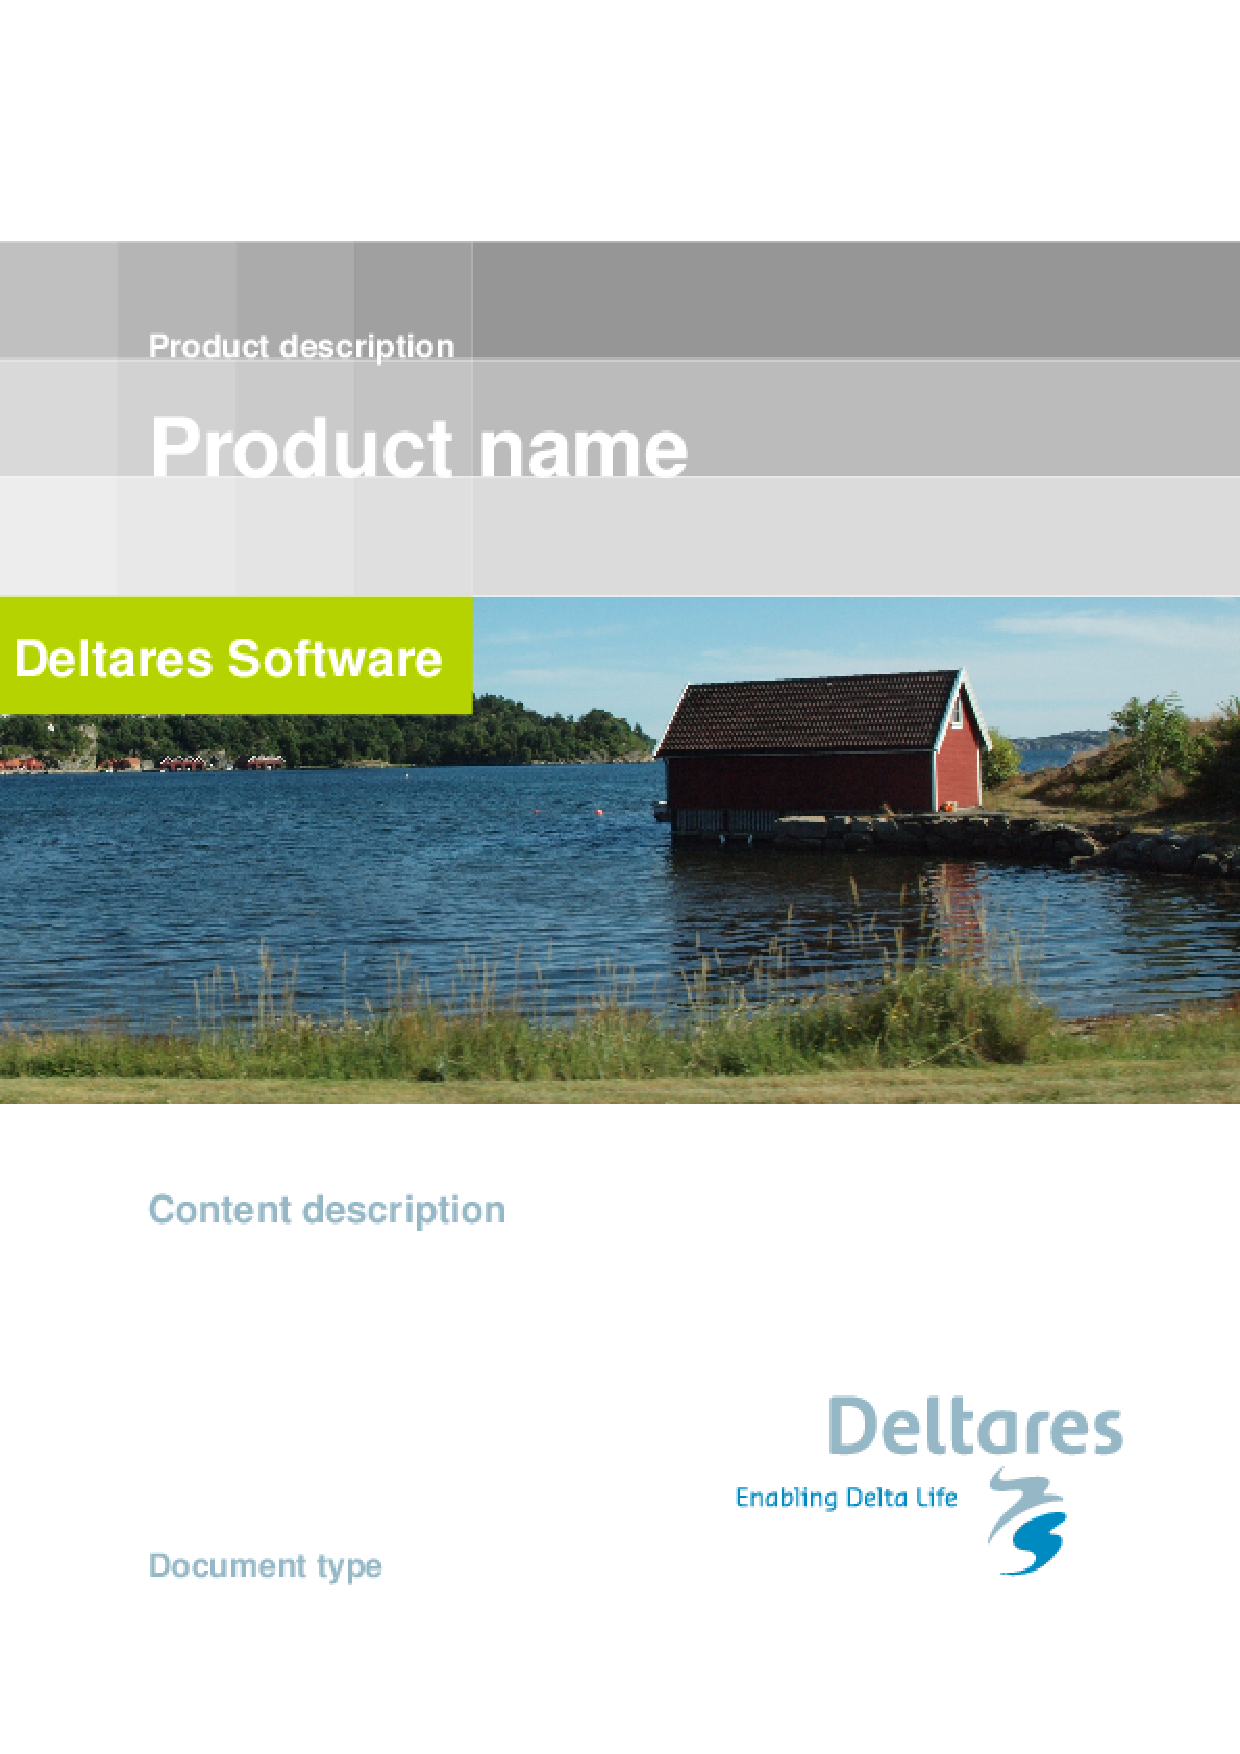
\includepdf[pages=1,offset=72 -70]{cover/default-cover-pages.pdf} % links-rechts past precies
\cleardoublepage

\title{Ringtoets}
\subtitle{}
\manualtype{Gebruikershandleiding}
\version{1.0}
\date{1 november 2015}
\manualtitle

\input{chapters/rt_guide}
\svnid{$Id: rt_installation.tex 1 2015-08-30 15:39:28Z rodriqu_dd $}

\chapter{Installatie\label{chap:install}}

\section{Inleiding}
Deze sectie beschrijft de installatie procedure van de applicatie Ringtoets. Hiervoor is in ieder geval het installatie bestand (Ringtoets Setup*.msi) nodig. Daarnaast worden er enkele eisen aan het besturingssysteem gesteld (zie \Autoref{sec:sysrequirements}). 

\section{Systeemeisen}
\label{sec:sysrequirements}
Voor een goed functioneren van RT is het wenselijk (of in sommige gevallen nodig) om een computer te hebben die minimaal voldoet aan de volgende eisen:
\begin{itemize}
	\item Microsoft Windows 7 hoger
	\item Microsoft .NET Framework versie 4.0 of hoger
	\item Minimaal een Intel Pentium III/800 MHz processor (of vergelijkbaar)
	\item Minimaal 256(???) MB RAM (1 GB RAM aanbevolen)
	\item Minimale beeldscherm resolutie van 1024x768 pixels
\end{itemize}




\section{RT installeren en opstarten}
\label{sec:rtinstall}
De installatie procedure wordt opgestart door op de snelkoppeling dubbel te klikken. Op bijna elke stap kan de procedure voortgezet worden door te drukken op \textit{Volgende}. De eerdere stap van de procedure kan bereikt worden door te klikken op \textit{Vorige}. Door op \textit{Annuleren} te klikken, kan de installatie onderbroken worden. 

Er zijn drie type installaties:
\begin{itemize}
	\item \textbf{Standaard}: de meest gebruikte onderdelen van het programma worden ge\"installeerd. Het programma wordt ge\"installeerd in de map
		
		\dir{C:\textbackslash Program Files (x86)\textbackslash Deltares\textbackslash Wettelijk Toets Instrumentarium (\color[rgb]{0.75,0.75,0.75}versienummer\color[rgb]{0,0,0})}.
		
		Dit is de aanbevolen optie voor de meeste gebruikers.
	\item \textbf{Aangepast}: de te installeren onderdelen en de map waarin het programma zal ge\"installeerd worden, kunnen geselecteerd worden. Door deze optie te kiezen, kan het ook gecontroleerd worden hoe veel ruimte de installatie in beslag zal nemen, en hoe veel ruimte beschikbaar is in de beschikbare volumes.
	\item \textbf{Volledig}: alle onderdelen van het programma worden ge\"installeerd. Het programma wordt ge\"installeerd in de map
		
		\dir{C:\textbackslash Program Files (x86)\textbackslash Deltares\textbackslash Wettelijk Toets Instrumentarium (\color[rgb]{0.75,0.75,0.75}versienummer\color[rgb]{0,0,0})}.
\end{itemize}

Op het moment dat de de installatietype gekozen is, wordt deze daadwerkelijk uitgevoerd door op \textit{Installeren} te klikken. De voortgang van de installatie wordt aangegeven totdat hij klaar is. Op dat moment wordt de installatie procedure volledig afgerond door op \textit{Voltooien}  te klikken.


Als het installatiebestand opgestart wordt nadat het programma ge\"installeerd is, kan de installatie aangepast worden. De mogelijke aanpassingen zijn:
\begin{itemize}
	\item \textbf{Wijzigen}: hiermee kan men opnieuw aangegeven worden welke onderdelen van het programma ge\"installeerd zullen zijn. 
	\item \textbf{Herstellen}: deze optie herstelt de ontbrekende of beschadigde bestanden, snelkoppelingen en registervermeldingen van de huidige installatie.
	\item \textbf{Verwijderen}: de installatie van het Wettelijk Toets Instrumentarium wordt volledig verwijderd van de computer door deze optie te kiezen.
\end{itemize}

Na installatie (\Autoref{sec:rtinstall}) kan Ringtoets worden opgestart via het startmenu (onder de map Deltares) of door op het bijbehorende icoontje (\Fref{fig:figinstall.1}) op het bureaublad dubbel te klikken. 


\begin{figure} [H]
	\centering
		\includegraphics{figures/chapter_installation/rt_desktop_icon}
	\caption{Ringtoets snelkoppelingsicoon op het bureaublad.}
	\label{fig:figinstall.1}
\end{figure}

Er wordt ook een snelkoppeling aangemaakt in het startmenu van Windows. Deze is te vinden in Startmenu $\,\to\,$ Alle programma's $\,\to\,$ Deltares $\,\to\,$ Ringtoets $\,\to\,$ Ringtoets:


\begin{figure} [H]
	\centering
		\includegraphics{figures/chapter_installation/rtInAllPrograms}
	\caption{Ringtoets in de startmenustructuur van Windows \color[rgb]{1,0,0} \textbf{Needs to be updated!!!}\color[rgb]{0,0,0}.}
	\label{fig:figinstall.2}
\end{figure}


Kort nadat het programma ge\"instaleersd is, is deze snelkoppeling direct te vinden onder het startmenu:


\begin{figure} [H]
	\centering
		\includegraphics{figures/chapter_installation/rtDirectlyinStartMenu}
	\caption{Ringtoets direct in het startmenu van Windows \color[rgb]{1,0,0} \textbf{Needs to be updated!!!}\color[rgb]{0,0,0}.}
	\label{fig:figinstall.3}
\end{figure}














\input{chapters/rt_general}
%\input{chapters/rt_overview}
\svnid{$Id: rt_guide.tex 1 2015-08-30 15:39:28Z rodriqu_dd $}

\chapter{Piping\label{chap:piping}}

\section{Inleiding}
Dit hoofdstuk beschrijft de procedure om een piping berekening op te zetten en uit te voeren. 

\section{Toevoegen van een piping faalmechanisme}
\label{sec:addpiping}
Om een piping berekening uit te voeren, moet er allereerst een RT project aangemaakt zijn in het algemeen project. Een RT project wordt toegevoegd in het \textbf{Project} toolvenster. Door op het project met de rechter muisknop te klikken, en dan door voor de opties \textit{New} en vervolgens \textit{Item} te kiezen.

\begin{figure} [H]
	\centering
		\includegraphics{figures/chapter_piping/addNewProject}
	\caption{Nieuw item toevoegen.}
	\label{fig:fig5.1}
\end{figure}

In de dialoog die dan te zien is, moet er gekozen worden voor een RT project:

\begin{figure} [H]
	\centering
		\includegraphics{figures/chapter_piping/selectRTProject}
	\caption{Nieuw toe te voegen item is RT project.}
	\label{fig:fig5.2}
\end{figure}

Door gebruik te maken van het contextmenu van het RT project, kan er uiteindelijk een piping faalmechanisme toegevoegd worden.

\begin{figure} [H]
	\centering
		\includegraphics{figures/chapter_piping/addPipingMechanismToProject}
	\caption{Toevoeging van faalmechanisme Piping aan RT project.}
	\label{fig:fig5.3}
\end{figure}


\section{Opbouw van het faalmechanisme}

\begin{figure} [H]
	\centering
		%\includegraphics{figures/chapter_piping/OpbouwFaalmechanisme}
	\caption{Opbouw van het faalmechanisme}
	\label{fig:fig5.4}
\end{figure}

Het faalmechanisme kent 3 onderdelen:
\begin{enumerate}
\item \textbf{Ondergrondprofielen}. Door gebruik te maken van het contextmenu kan een .soil database met de stochastische schematisatie van de
ondergrond (SOS database) worden ge\"{i}mporteerd.
\item \textbf{Dwarsdoorsneden}. Door gebruik te maken van het contextmenu kan een .soil database met de stochastische schematisatie van de
ondergrond (SOS database) worden ge\"{i}mporteerd.
\item \textbf{Piping}. In het \textbf{Properties} venster kunnen de piping varaiabelen worden aangepast:
\begin{figure} [H]
	\centering
		%\includegraphics{figures/chapter_piping/PipingProperties}
	\caption{Aan te passen piping variabelen}
	\label{fig:fig5.5}
\end{figure}
	\begin{itemize}
	\item \textbf{Naam}: Naam van de berekening, door de gebruiker te wijzigen
	\item \textbf{Volumiek gewicht van water}: Het volumegewicht  $\gamma$ \textsubscript{water}  is ca. 10 kN/m\textsuperscript{3}
	\item \textbf{Modelfactor opbarsten}: Rekenwaarde van de modelonzekerheid
	\item \textbf{Toetspeil}: Het door HydraRing berekende toetspeil voor dit dijkvak
	\item \textbf{Stijghoogte bij uittredepunt}: 
	\item \textbf{Dempingsfactor bij uittredepunt}: Stochast; Relateert respons van stijghoogte bij binnenteen aan buitenwaterstand
	\item \textbf{Freatische waterstand bij uittredepunt}: Stochast; 
	\item \textbf{Stijghoogte in achterland}: 
	\item \textbf{Kritiek verhang m.b.t. heave}: Stochast; 
	\item \textbf{Totale deklaagdikte bij uittredepunt}: Stohast; Dikte van de laag boven de aquifer tot aan maaiveld of onderkant sloot
	\item \textbf{Modelfactor piping toegepast op Sellmeijermodel}: Rekenwaarde van de modelonzekerheid
	\item \textbf{Reductiefactor Sellmeijer}: 
	\item \textbf{Kwelweglengte}: De horizontale afstand tussen intrede- en uittredepunt die het kwelwater in de aquifer aflegt
	\item \textbf{Volumiek gewicht van de zandkorrels onder water}: Stochast; Het (ondergedompelde) volumegewicht van de korrels in de zandlaag.
	\item \textbf{Co\"{e}ffici\"{e}nt van White}: Sleepkrachtfactor volgens White
	\item \textbf{70\%-fraktiel van de korreldiameter in de bovenste zandlaag}: Stochast; Zeefmaat waar 70 gewichtsprocent van de korrels doorheen gaat. Hier de korreldiameter van het bovenste gedeelte van de aquifer, zonder de fijne fractie (<63$\mu$ meter)
	\item \textbf{Doorlatendheid aquifer}: Stochast; Darcy-snelheid waarmee water door de eerste zandlaag stroomt
	\item \textbf{Kinematische viscositeit van water bij 10\textsuperscript{$\circ$} Celsius}: 
	\item \textbf{Valversnelling}: Versnelling van de zwaartekracht [m/s\textsuperscript{2}] $\approx$ 9.81
	\item \textbf{Dikte watervoerend pakket}: Stochast; De dikte van de zandlaag die als aquifer is benoemd
	\item \textbf{Referentiewaarde voor 70\%-fraktiel in Sellmeijer regel}: Gemiddelde d70 van de in kleine schaalproeven toegepaste zandsoorten waarop de formule van Sellmeijer is gefit = 0.000208 meter
	\item \textbf{Rolweerstandshoek}: Hoek in het krachtenevenwicht die aangeeft hoeveel de korrels weerstand beiden tegen rollen; ook beddingshoek genoemd
	\begin{figure} [H]
	\centering
		%\includegraphics{figures/chapter_piping/PipingSurfacelines}
	\caption{Keuzemenu dwarsdoorsneden}
	\label{fig:fig5.6}
\end{figure}
	\item \textbf{Dwarsdoorsnede}: Keuzemenu om de dwarsdoorsnede die voor de pipingsom wordt gebruikt te selecteren die zijn opgehaald in het \textbf{Project} venster
	\item \textbf{Ondergrondprofiel}: Keuzemenu om het ondergrondprofiel die voor de pipingsom wordt gebruikt te selecteren die zijn opgehaald in het \textbf{Project} venster
	\end{itemize}

\end{enumerate}








Als alle invoergegevens voor een piping faalmechanisme berekening klaar zijn, kan deze uitgevoerd worden door op Berekenen te klikken in het contextmenu.

Als de berekening niet uitgevoerd kan worden, dan komt er een bericht terecht in het berichtpanel met verdere informatie over de reden dat het fout is gegaan. Als de berekening wel uitgevoerd is, is het resultaat toegevoegd (of ge\"{u}pdatet) in het projectpanel.








%\appendix
%\svnid{$Id: A_How_to_use_OpenDA_models.tex 1 2015-10-01 15:39:28Z rodriqu_dd $}

\chapter{Example of an appendix}\label{How_to_use_OpenDA_models}

%include text from common, as this is shared with the Delta Shell User Manual
\svnid{$Id: Appendix1_text.tex 1 2015-08-30 15:39:28Z rodriqu_dd $}

%this text can be shared between several User Manuals

\section{Introduction} \label{sec:Appendix1Intro}

Here goes the introduction to this appendix. 
\section{Second section of this appendix} \label{sec:Appendix1Section2}

\subsection{Subsection in second section of this appendix}

Blah, blah, blah,...


\subsection{And another subsection}

With more text in here.

\section{Last section}

The text of the last section.



\cleardoublepage
%
\newpage
\pagestyle{empty}
\mbox{}
\includepdf[pages=2,offset=-72 -70]{cover/default-cover-pages.pdf} % links-rechts past precies
\end{document}